\section{Architecture}\label{sec:architecture}

In this section, we will detail the architecture of our implementation.
\autoref{fig:component-diagram} provides a rough overview of our project's architecture.
It uses UML-like syntax to highlight the core components of the module and its interfaces between each other
and the outer world.
Each of these components are explained in detail in the following subsections.

\begin{figure*}[h!]
    \centering
    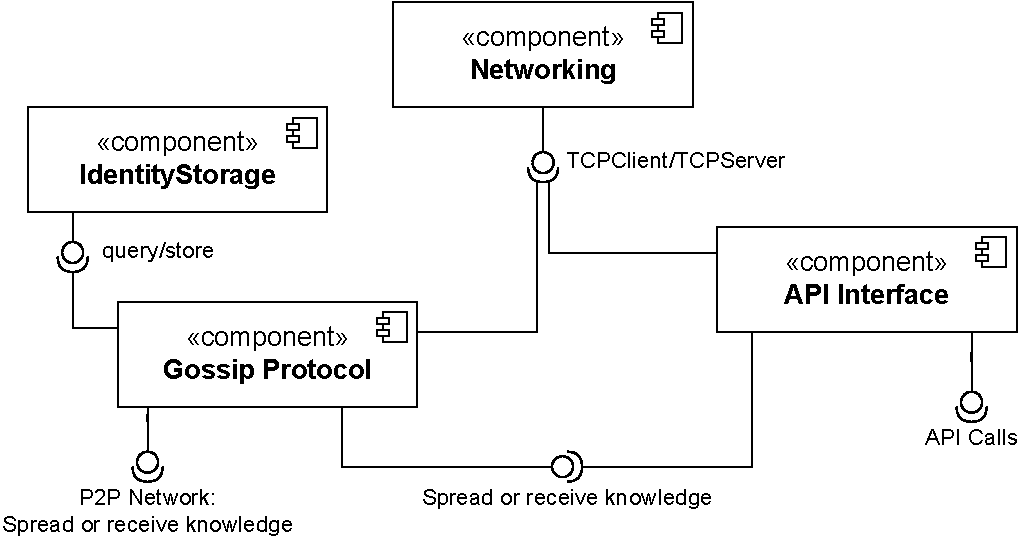
\includegraphics[width=1\linewidth, angle=0]{images/Components-Gossip}
    \caption{UML-like component diagram depicting a rough subsystem decomposition of our system.
    It highlights the fundamental structure and architecture of our project.}
    \label{fig:component-diagram}
\end{figure*}

\subsection{Networking}\label{subsec:networking}

The \textbf{Networking} component is built on top of the \textit{Netty 4}\footnote{https://netty.io} networking framework.
It provides common abstractions used by both the API and the Gossip component.
Namely, it handles packet encoding and decoding, and connection establishment.

Packet serialization and deserialization can be implemented by conforming to the \ttt{OutboundPacket} or
\ttt{InboundPacket} interfaces (defining a respective \ttt{InboundPacketHandler}, respectively).
The set of supported packets can then be built using \ttt{ProtocolDescription} by supplying the packet
implementations and their corresponding packet ids.

Together with an \ttt{EventLoopGroup} instance, \ttt{ProtocolDescription}s can be used to instantiate
a \ttt{TCPClient} or \ttt{TCPServer} to bind the respective TCP socket.
\ttt{EventLoopGroup}\footnote{https://netty.io/4.1/api/io/netty/channel/EventLoopGroup.html}
is a concept provided by Netty, which manages a thread pool to handle incoming connections and
serialization of traffic asynchronously.

\subsubsection{Common Packet Format}

The \ttt{ConnectionInitializer} (automatically set up within the \ttt{TCPClient} or the \ttt{TCPServer})
constructs the channel pipeline for each connection.
The resulting channel pipeline is depicted in \autoref{fig:channel-pipeline}.
Incoming traffic passes through the \ttt{LengthFieldBasedFrameDecoder}\footnote{Provided by Netty: https://netty.io/4.1/api/io/netty/handler/codec/LengthFieldBasedFrameDecoder.html}
(parsing the \textit{size} field) and the \ttt{PacketDecoder} (parsing the \textit{packet id}, assembling the typed packet instances)
to the \ttt{InboundHandler}, calling the corresponding user code to handle the packet.
Outbound traffic passes the \ttt{PacketEncoder} (serializing the packet contents and writing the \textit{packet id})
and the \ttt{LengthFieldPrepender} (writing the \textit{size} field).

The illustrated channel pipeline results in the general packet header depicted in \autoref{fig:basic-packet-layout}.
The \textit{size} field is an unsigned 16-bit integer, resulting in a maximum packet size of
65535 bytes (including the header size).

\begin{figure*}[h!]
    \centering
    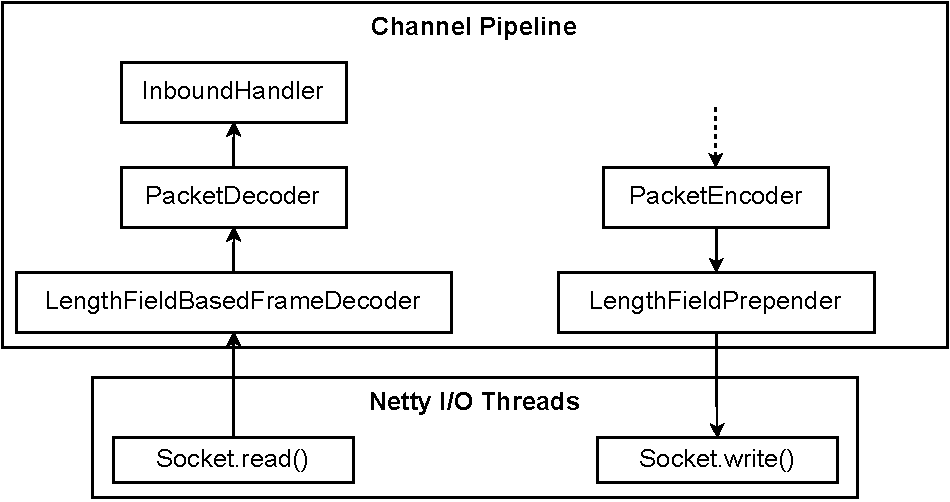
\includegraphics[width=1\linewidth, angle=0]{images/ChannelPipeline}
    \caption{Diagram of the Channel Pipeline of an open connection.}
    \label{fig:channel-pipeline}
\end{figure*}

\begin{figure}
    \centering
    \begin{bytefield}{32}
        \bitheader{0,7-8,15-16,23-24,30-31} \\
        \begin{rightwordgroup}{Packet \\  Header}
            \bitbox{16}{size} & \bitbox{16}{\texttt{packet Id}}
        \end{rightwordgroup} \\
        \begin{rightwordgroup}{Packet \\ Payload}
            \wordbox[tlr]{1}{} \\
            \skippedwords \\
            \wordbox[lrb]{1}{}
        \end{rightwordgroup}
    \end{bytefield}
    \caption{Packet header layout used within all packet types.}
    \label{fig:basic-packet-layout}
\end{figure}

\subsection{API Interface}\label{subsec:api-interface}

The \textbf{API Interface} implements the TCP socket-based API used by other modules to interact with Gossip (see \autoref{sec:requirements}).
Packet definitions are provided for the four API messages
\ttt{ANNOUNCE}, \ttt{NOTIFY}, \ttt{NOTIFICATION}, and \ttt{VALIDATION}, as outlined in the specification.
The component relies on the networking abstractions introduced in \autoref{subsec:networking}.

Incoming API message calls are forwarded to the \ttt{GossipModule}, which is part of the \textit{Gossip Protocol} component.
The module is provided with a connection handle to send out potential notifications later.

\subsection{Gossip Protocol}\label{subsec:gossip-protocol}

The \textbf{Gossip Protocol} component implements the protocol spoken between individual Gossip peers.
We rely on TCP to create a strongly connected network and rely on retransmissions and congestion control.

As outlined in the project specification, hostkeys are distributed out-of-band.
Therefore, we currently don't consider identity exchange (see \autoref{subsec:gossip-protocol-future-work}).
Known identities with their respective public keys and last known connection information are stored
on disk inside the \ttt{identities} folder controlled by the \textbf{IdentityStorage} component.
For testing purposes, we supply the \ttt{generateHostKey.sh} script to generate hostkeys for testing purposes.
Further, the command line interface of our application provides means to generate and import identities in the
required format (refer to the \ttt{README.md} for more information).

Our protocol consists of two phases, the initial \textit{handshake} phase and the \textit{knowledge-spreading} phase
for established connections.
The \ttt{DISCONNECT} is the only packet valid in both phases and which might be sent at any time.
Its structure is depicted in \autoref{fig:gossip-packet-disconnect}.
It consists of a single \textit{reason} field describing the disconnect reason.
We currently maintain the following possible reasons: \ttt{NORMAL(0)}, \ttt{UNSUPPORTED(1)}, \ttt{AUTHENTICATION(64)},
\ttt{UNEXPECTED\_FAILURE(65)}, \ttt{CANCELLED(66)}, \ttt{DUPLICATE(67)}, \ttt{BUSY(68)}, \ttt{NOT\_ALLOWED(69)}
and \ttt{TIMEOUT(70)}.
Please derive their exact meaning from the technical documentation of the \ttt{GossipPacketDisconnect.Reason} class.

\begin{figure}[h!]
    \centering
    \begin{bytefield}{32}
        \bitheader{0,7-8,15-16,23-24,30-31} \\
        \bitbox{16}{size} & \bitbox{16}{\texttt{DISCONNECT}}\\
        \bitbox{8}{reason} & \bitbox{24}{reserved} \\
    \end{bytefield}
    \caption{GossipPacketDisconnect}
    \label{fig:gossip-packet-disconnect}
\end{figure}

The two protocol phases are described in detail in the following two subsections.

\subsubsection{Handshake}

For the handshake, we recall the requirements set in \autoref{sec:requirements}.
The primary purpose of the handshake is to create a secure channel for communication and verify
and authenticate identity claims of the peers mutually.

We rely on \textit{TLS 1.3}, serving us with a reliable, secure, and well-tested secure channel implementation.
Consequentially, we employ ECDHE (Elliptic Curve Diffie Hellman with an Ephemeral key) for the key exchange,
providing perfect forward secrecy for ongoing traffic.
For application-data, encryption we configure the AEAD cipher \textit{ChaCha20-Poly1305} supporting our confidentiality
and integrity security goals.

Our TLS layer is configured to do mutual authentication, meaning both the server and the client provide respective
certificates.
The root of trust for a peer's certificate chain is derived from its hostkey (a self-signed certificate containing
the public part of the hostkey).
This certificate acts as a Certificate Authority to an intermediate certificate used within the TLS authentication phase.
Within our \ttt{TrustManager} implementation, we verify the integrity of the certificate chain and ensure that
the root certificate is self-signed with the expected hostkey identity.
Certificate transmissions are encrypted with TLS 1.3.
Therefore, this doesn't leak the peer's identity at the connection establishment.
Each peer verifies that the TLS session was established with the expected hostkey ensuring that no man-in-the-middle
attack is in progress.

After completing the TLS handshake, we continue with the gossip handshake used to establish our application-domain-specific
constraints and expectations.

\paragraph{Handshake Hello}

After the TLS handshake completes, the connection-initiating peer sends the
\ttt{HANDSHAKE HELLO} (see \autoref{fig:gossip-packet-handshake-hello}) packet to the server.
The packet specifies the used protocol \textit{version} (currently always \ttt{VERSION\_1(1)}).
While the packet does not transport any elementary information, it marks the explicit begin of the gossip protocol.

Upon receiving the packet, we check our local identity storage, to ensure that we only accept connections from peers
that are part of our identity storage.
Further, we verify, that the remote peer's ip address matches the expected ip address of the locally stored identity
(established out-of-band as explained \autoref{sec:requirements}).
A future version of our Gossip implementation might employ a Proof-of-Work (PoW) mechanism to update the expected ip address to
provide a more robust peer-to-peer network implementation (see \autoref{sec:future-work}).
Lastly, we impose rate limiting on the amount of connection attempts that can be made from the same ip address.
This is to reduce the attack surface of Sybill attacks, making it harder to stage such attacks from a single machine.

\begin{figure}[h!]
    \centering
    \begin{bytefield}{32}
        \bitheader{0,7-8,15-16,23-24,30-31} \\
        \bitbox{16}{size} & \bitbox{16}{\texttt{HANDSHAKE HELLO}}\\
        \bitbox{8}{version} & \bitbox{24}{reserved} \\
    \end{bytefield}
    \caption{GossipPacketHandshakeHello}
    \label{fig:gossip-packet-handshake-hello}
\end{figure}

\paragraph{Handshake Complete}

The \ttt{HANDSHAKE COMPLETE} (\autoref{fig:gossip-packet-handshake-complete}) is the explicit signal to the client
that the previous validation steps were successful and that the client
should also switch to the \textit{Knowledge Spreading} phase.
The packet does not have any contents.

\begin{figure}[h!]
    \centering
    \begin{bytefield}{32}
        \bitheader{0,7-8,15-16,23-24,30-31} \\
        \bitbox{16}{size} & \bitbox{16}{\texttt{HANDSHAKE COMPLETE}}\\
    \end{bytefield}
    \caption{GossipPacketHandshakeComplete}
    \label{fig:gossip-packet-handshake-complete}
\end{figure}

\subsubsection{Knowledge Spreading}

Once clients complete the \textit{Handshake} phase, they reside in the \textit{Knowledge Spreading} phase
and are active participants in the Gossip peer-to-peer network.

Once an API consumer subscribes to a data type (see \autoref{subsec:api-interface}), it may announce
data into the network.
To do so, we overtime propagate the \ttt{SPREAD KNOWLEDGE} packet to all connected peers (see \autoref{fig:gossip-spread-knowledge}).
For each announced data point, we generate a random 64-bit \textit{message id}.
In combination with the \textit{ttl} field (defined by the API consumer and decremented at every hop),
it provides means to avoid cycles in packet routing.

On arrival of a \ttt{SPREAD KNOWLEDGE}, we provide the data contents to all API connections subscribed to the
data type.
If there are none, we discard the packet.
Otherwise, we only forward the packet further into the network if all subscribed API connections report
validity of the packet contents.
This ensures that we don't propagate manipulated information into the network.

We impose some rate limiting restrictions on the amount of knowledge a remote peer can spread into the network.
This is to reduce the attack surface on potential denial-of-service attacks (e.g., by changing the message id).

\begin{figure}[h!]
    \centering
    \begin{bytefield}{32}
        \bitheader{0,7-8,15-16,23-24,30-31} \\
        \bitbox{16}{size} & \bitbox{16}{\texttt{SPREAD KNOWLEDGE}}\\
        \wordbox[tlr]{1}{message id} \\
        \wordbox[lrb]{1}{} \\
        \bitbox{16}{ttl} & \bitbox{16}{data type} \\
        \bitbox{32}{reserved} \\
        \wordbox[tlr]{1}{data} \\
        \skippedwords \\
        \wordbox[lrb]{1}{}
    \end{bytefield}
    \caption{GossipPacketSpreadKnowledge}
    \label{fig:gossip-spread-knowledge}
\end{figure}

